\chapter{Continuous Distributions}


\section{Continuous Probability Distributions}
What is the probability that a newborn weighs exactly 3.4 kg? Not 3.4001,
not 3.3999, but exactly 3.4000000\ldots? The answer is zero, and yet babies
are born near 3.4 kg all the time. Continuous quantities need a new way of
thinking about probability.

When we talked about the probability distribution of the sum of two dice,  we assigned a probability to each of the 11 possibilities:
\begin{figure}[H]
    \centering
    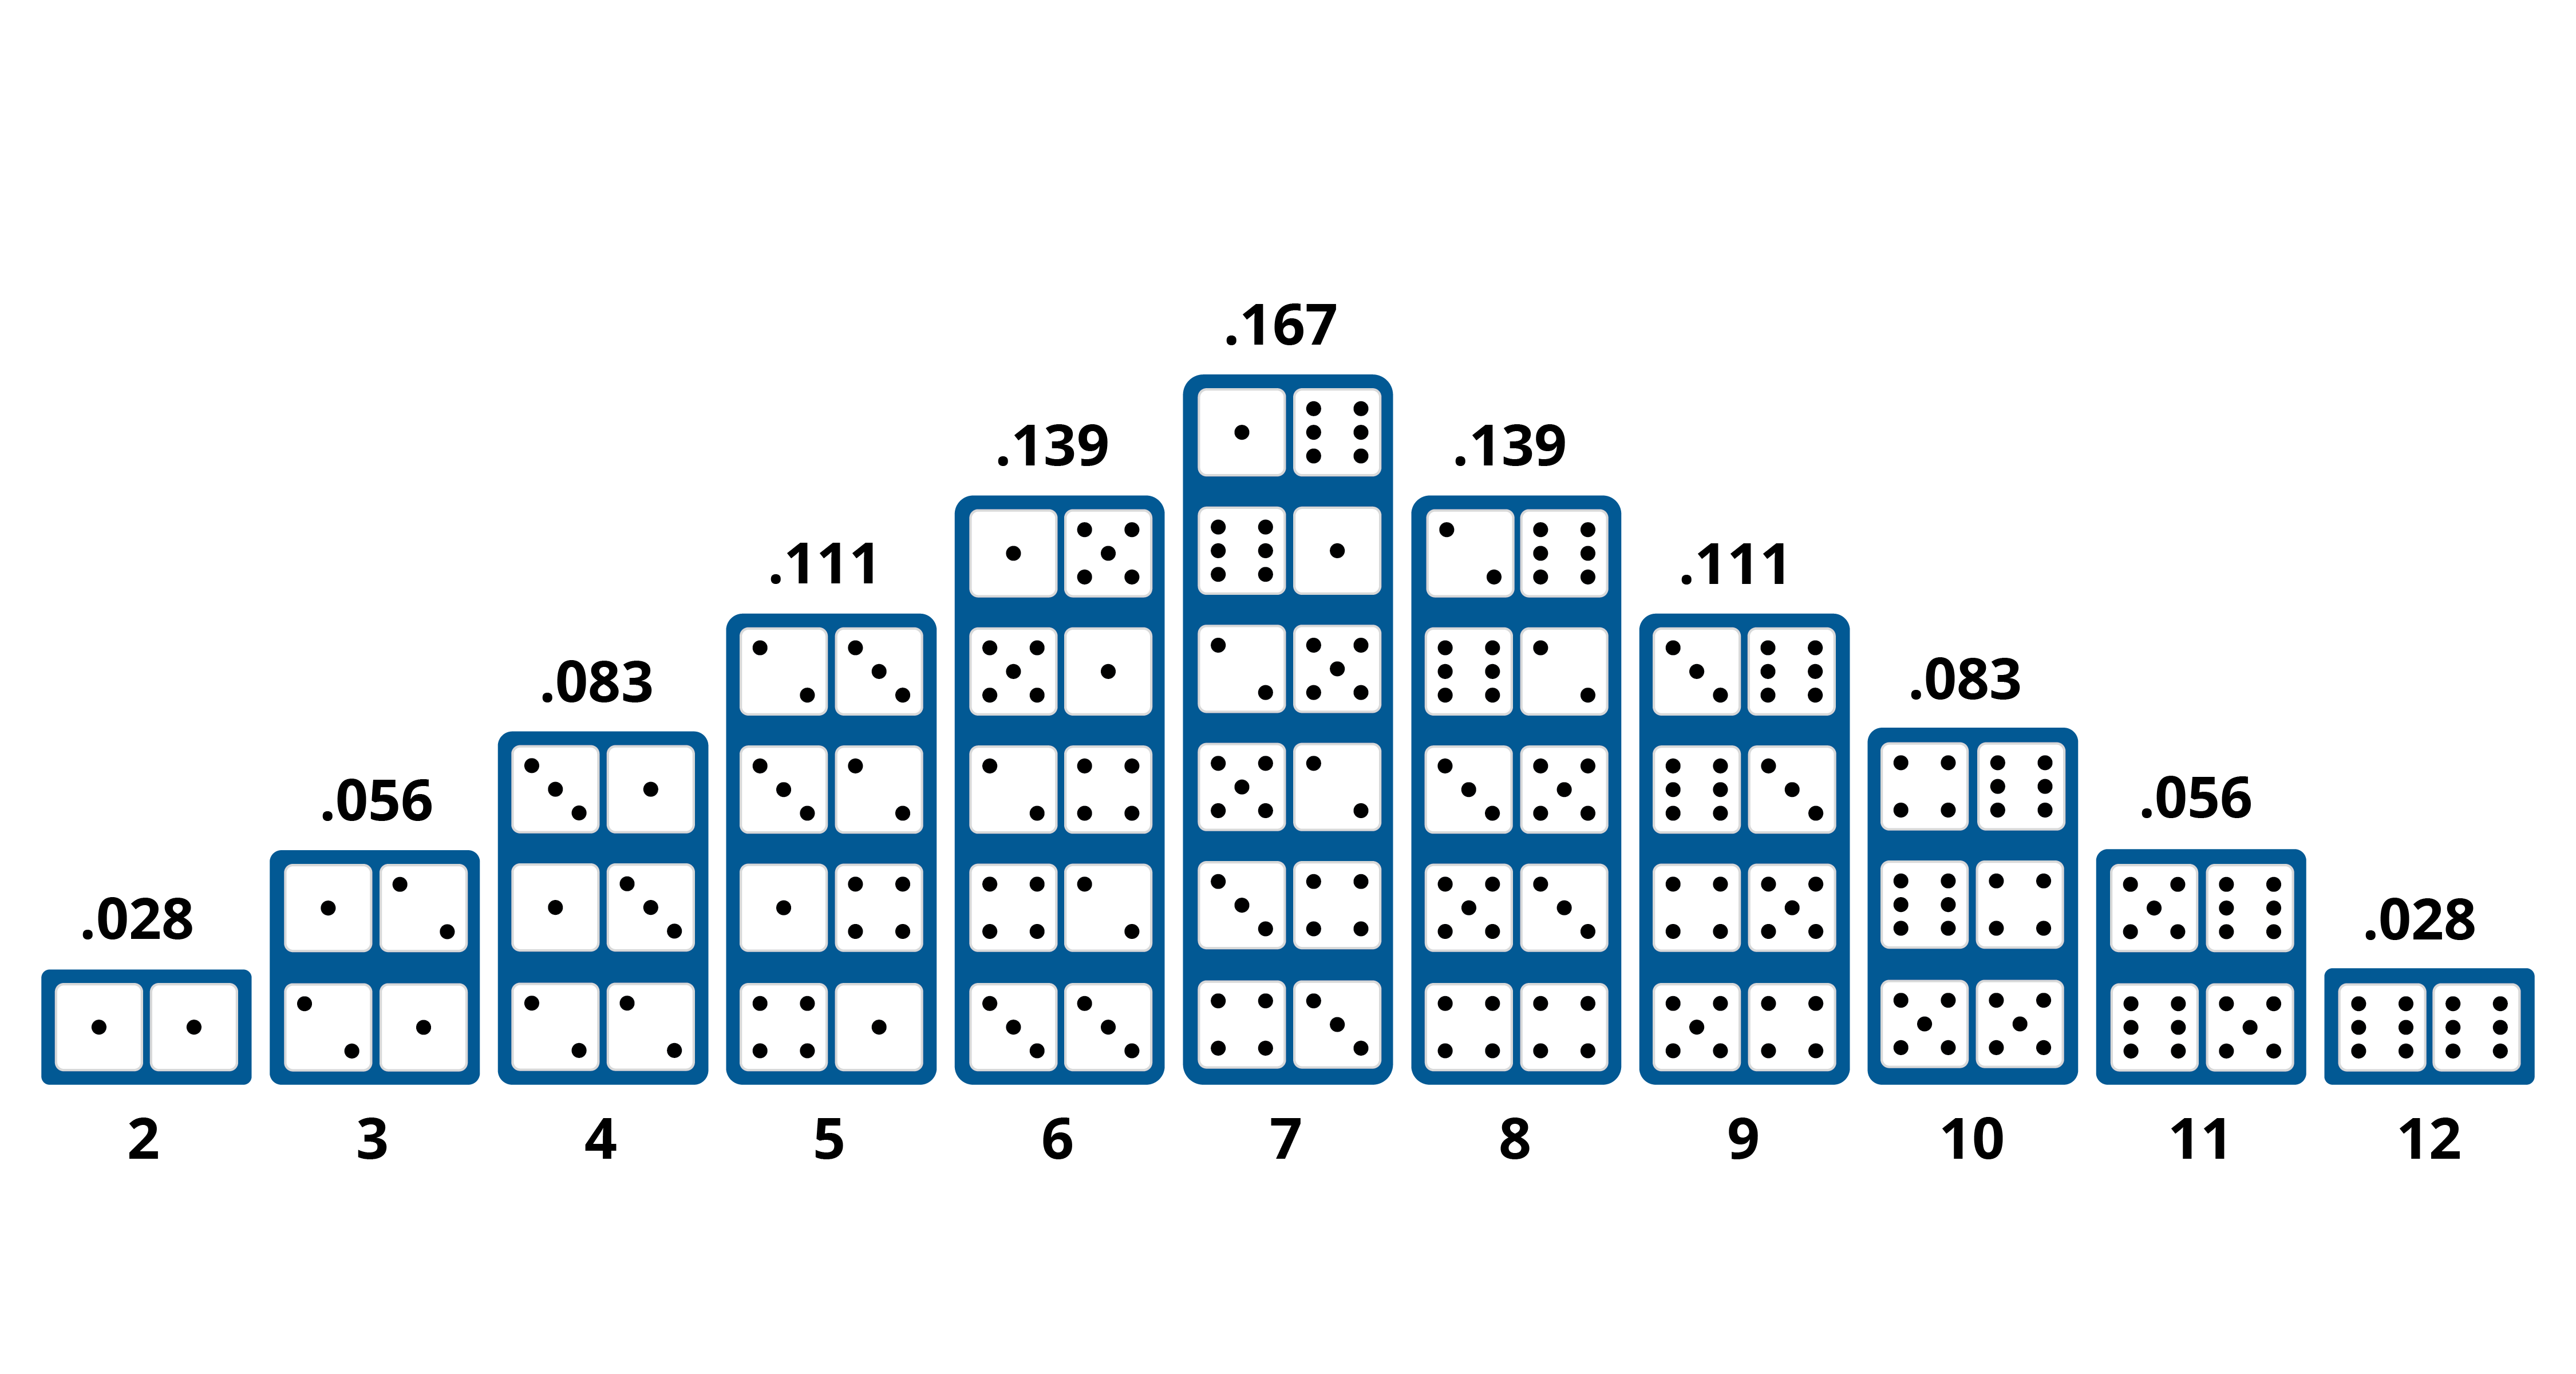
\includegraphics[width=0.7\textwidth]{dice_histogram.png}
    \caption{Rolling two dice probability distribution.}
    \label{fig:example-continuous_distributions}
\end{figure}

The probabilities all added up to be 1.0. That is a way of saying ``100\% of the times you throw the dice,  the sum will be an integer between 2 and 12.''

Now we need to talk about probabilities of properties that are continuous,  not discrete. For example, we might want to ask the question, ``If I randomly pick a cow from all the cows in the 
world, what is the probability that it will weigh less than 597.34 kg?''  What does a probability distribution for a continuous variable look like?

\subsection{Cumulative Distribution Function}

Imagine that you live in ancient times. You buy, sell, and ship cows. A lot of people come into your office and brag about their cows: "Bessie is heavier than 99\% of the cows in 
world!"  So, you need to develop some statistics on cow weights.

You have ten cows. You weigh them:

\begin{tabular}{c|r}
Cow & Mass in kg \\
\hline
Cow 1 & 580.22 \\
Cow 2 & 540.07 \\
Cow 3 & 538.20 \\
Cow 4 & 512.39 \\
Cow 5 & 589.75 \\
Cow 6 & 456.91 \\
Cow 7 & 583.09 \\
Cow 8 & 493.56 \\
Cow 9 & 489.97 \\
Cow 10 & 704.15 \\
\end{tabular}

If someone comes into your shop and says, ``My Bessie is an astonishing 530 kg!'' it would be cool to have a list on the wall that would let you yell back, ``Most of my cows are heavier than that, Silly!''  So, you sort the cows by weight. For each weight,  you say how many of your cows are lighter than that:

\begin{tabular}{c|r}
Proportion of cows lighter & Mass in kg \\
\hline
0.00 & 456.91 \\
0.10 & 489.97 \\
0.20 & 493.56 \\
0.30 & 512.39 \\
0.40 & 538.20 \\
0.50 & 540.07 \\
0.60 & 580.22 \\
0.70 & 583.09 \\
0.80 & 589.75 \\
0.90 & 704.15 \\
\end{tabular}

In fact, for easy reference,  you make a plot:
\begin{figure}[H]
    \centering
    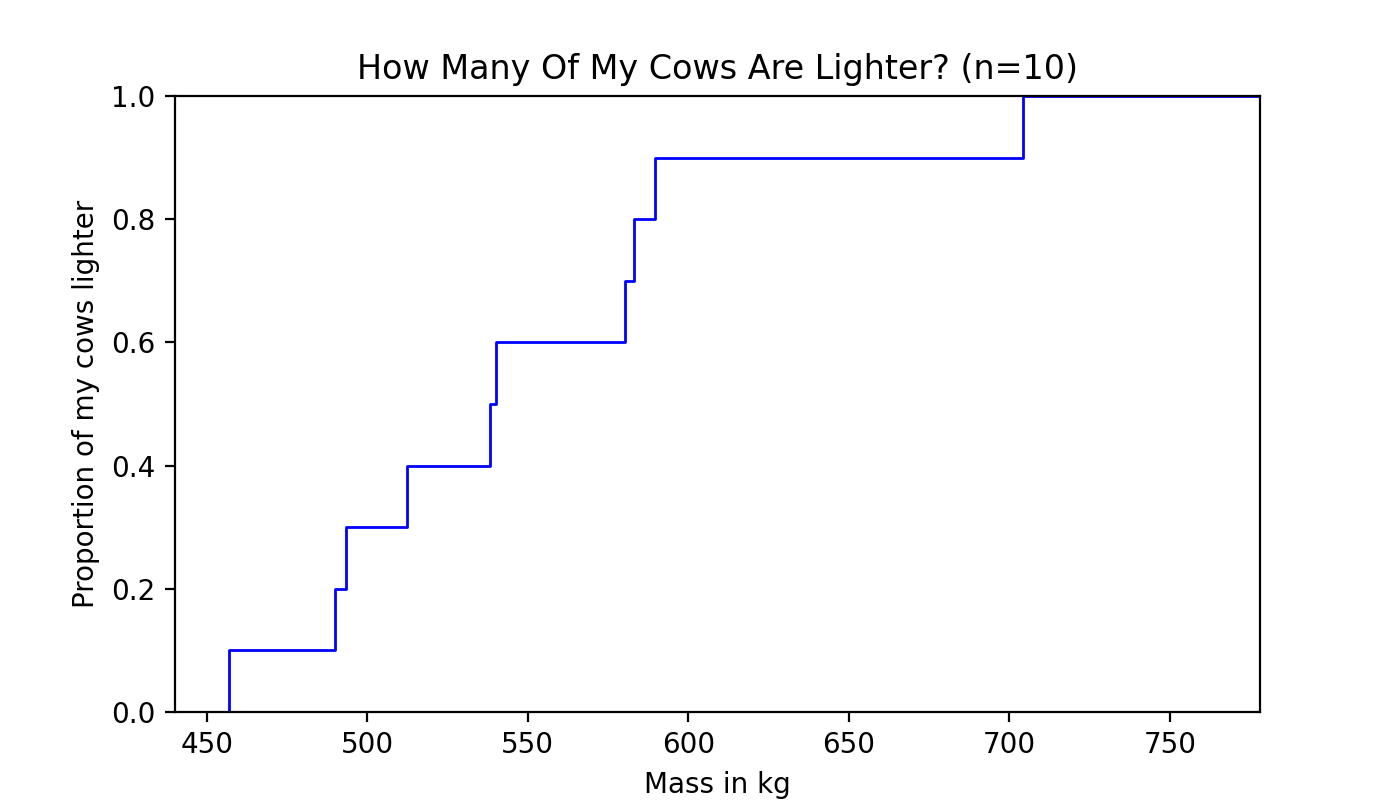
\includegraphics[width=0.7\textwidth]{cow_sample_cdf.png}
    \caption{10 cow cumulative distribution function.}
    \label{fig:10cdf}
\end{figure}

Now, for any weight, you can quickly look up what proportion of your cows are lighter (and, if you subtract that from 1,  what proportion of your cows are heavier).

See how jagged that graph is?  That is because you only have the data for 10 cows. However, as the years pass and you weigh thousands of cows, the plot will become smoother. Because it
always accumulates more cows as you move from left to right, this is known as a \newterm{cumulative distribution function}, or CDF:\index{cumulative distribution function}
\begin{figure}[H]
    \centering
    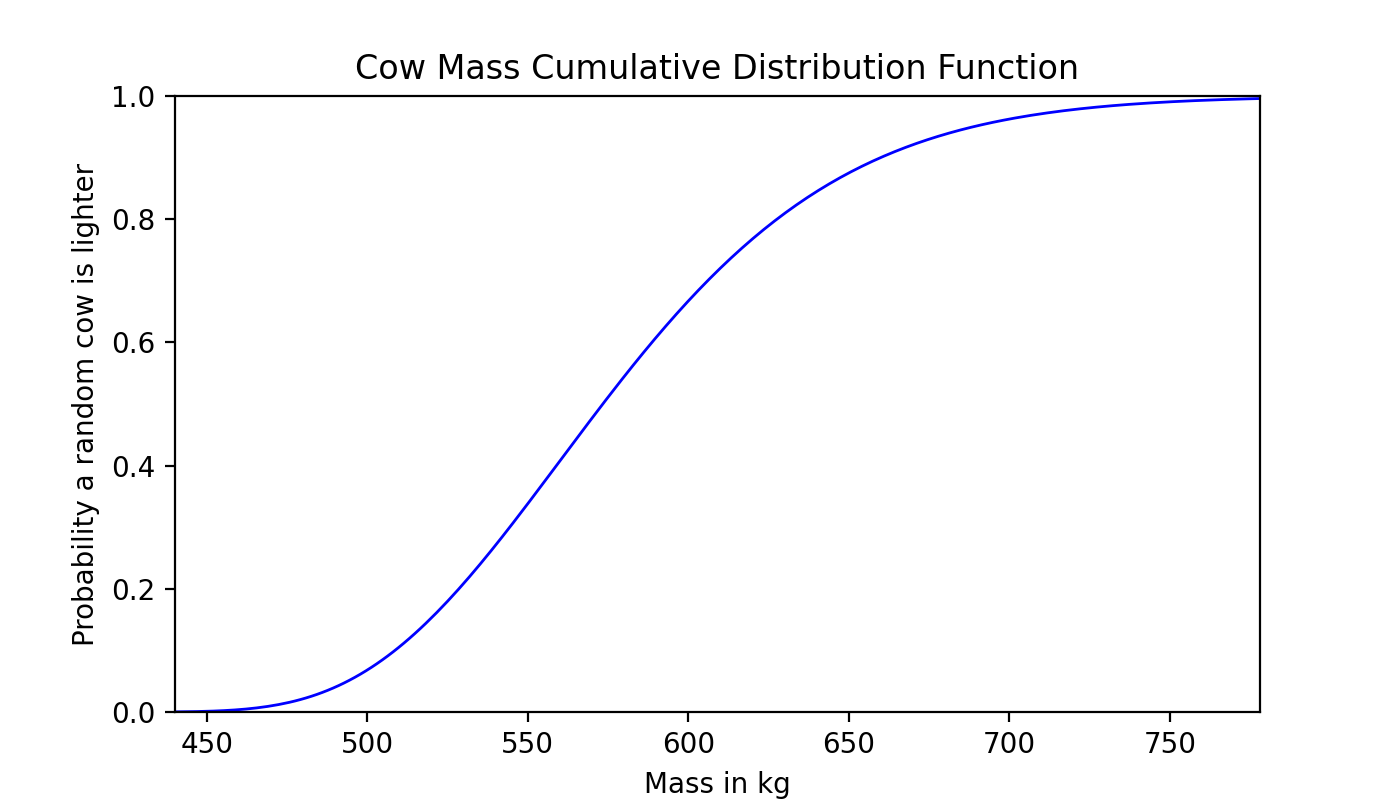
\includegraphics[width=0.7\textwidth]{cow_cdf.png}
    \caption{Cumulative distribution function for cow weights.}
    \label{fig:cowcdf}
\end{figure}

A cumulative distribution function always starts at 0 and ends at 1. On that journey, it never decreases. Reading the graph tells you what proportion of the population is \emph{less than} any given value. For bell-shaped data, the CDF is an S-shaped curve: flat at the ends and steepest in the middle, where most of the values are. 

Let us say you want to know what proportion of cows weigh between 620 kg and 635 kg. Using the CDF, you could figure out that 77\% of all cows weigh less than 620 kg and 83\% of all cows 
weigh less than 635 kg. Thus 6\% of all cows must weigh more than 620 kg and less than 635 kg.
\begin{figure}[H]
    \centering
    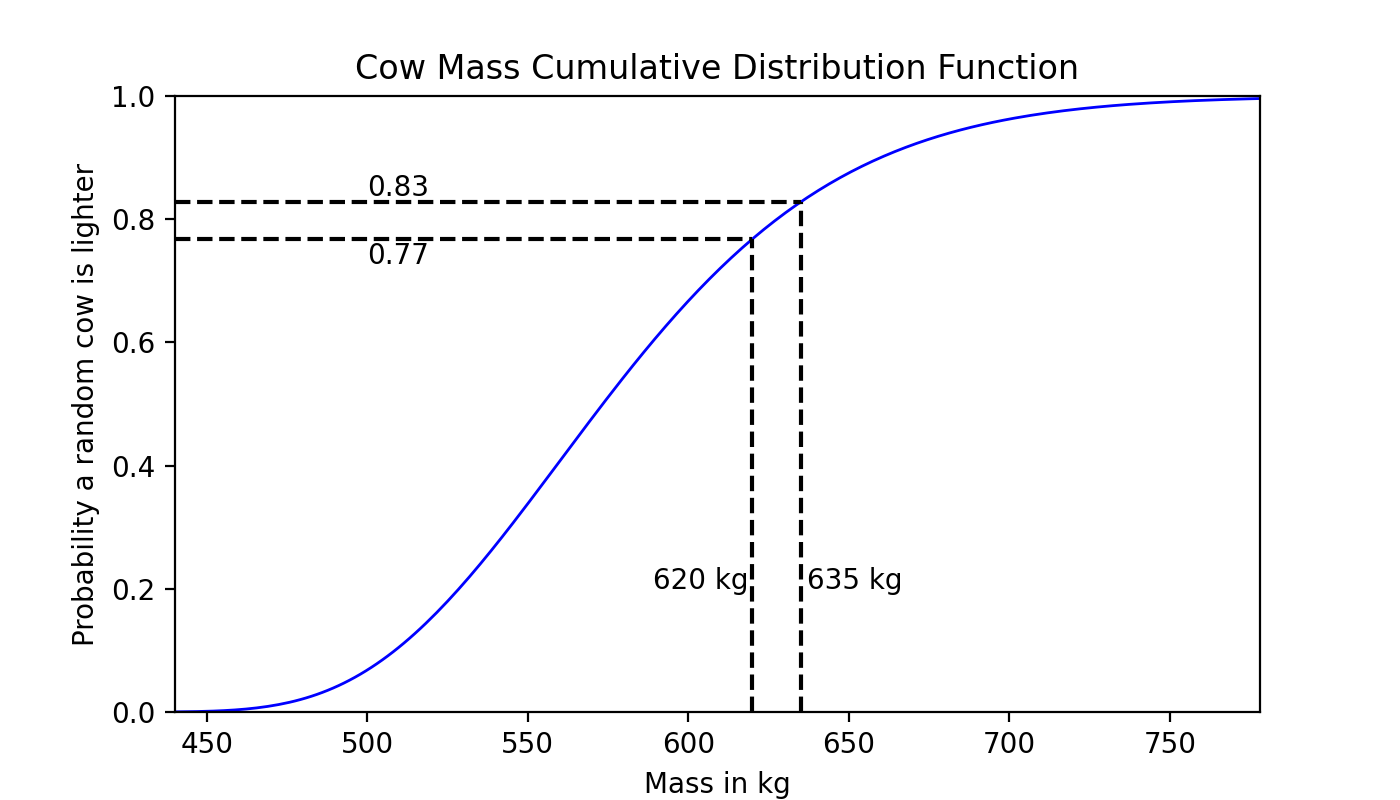
\includegraphics[width=0.7\textwidth]{cow_cdf_bounds.png}
    \caption{Cumulative distribution function with bounds from 620 kg to 635 kg.}
    \label{fig:cowcdfbounds}
\end{figure}

\subsection{Probability Density Function}
\index{probability density function}
The cumulative distribution function is handy,  but some of its information can be hard to see. For example, how would you answer the question, ``What is the most common weight of a cow?"  You would
squint at the CDF and try to determine where it was steepest.

To make these sorts of questions easier to answer,  we take the derivative of the CDF to get the \newterm{probability density function} (or PDF). For the cows,  it would look like this:
\begin{figure}[H]
    \centering
    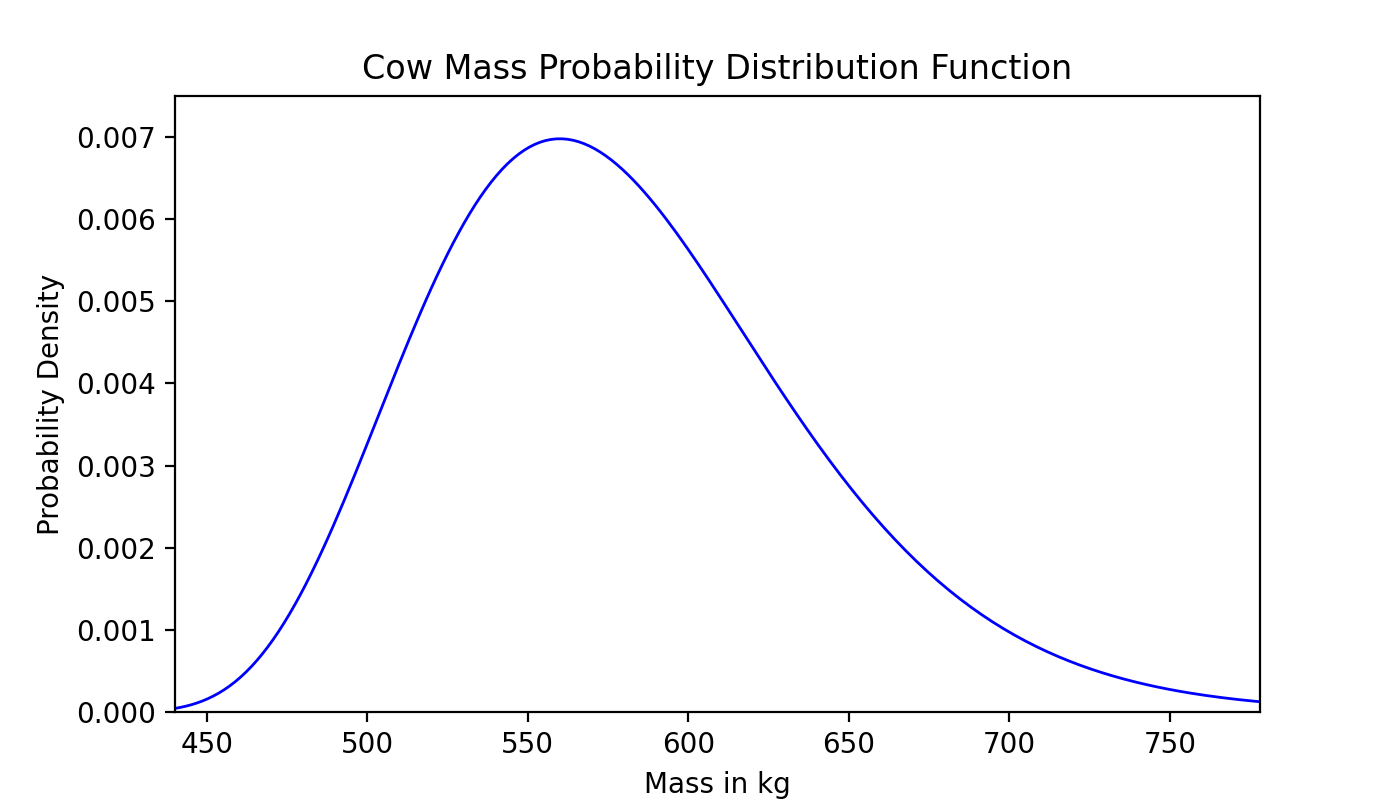
\includegraphics[width=0.7\textwidth]{cow_pdf.png}
    \caption{Probability density function for cow weights.}
    \label{fig:cowpdf}
\end{figure}

Now you can easily see that the CDF was steepest at about 560 kg. The value where the PDF is highest is called the \newterm{mode}: the most common weight. You might say ``560 kg is the mode of cow mass.'' \index{mode}

Note that the mode is often different from the mean or the median. In this case, for example,  the distribution is skewed right --- the long tail of heavy cows pulls the mean and median above the mode.

Once again,  let us say you want to know what proportion of cows weigh between 620 kg and 635 kg. This is more difficult with a PDF than it is with a CDF. With a PDF,  you have to find
the area under the curve between $x=620$ and $x=635$. 

\begin{figure}[H]
    \centering
    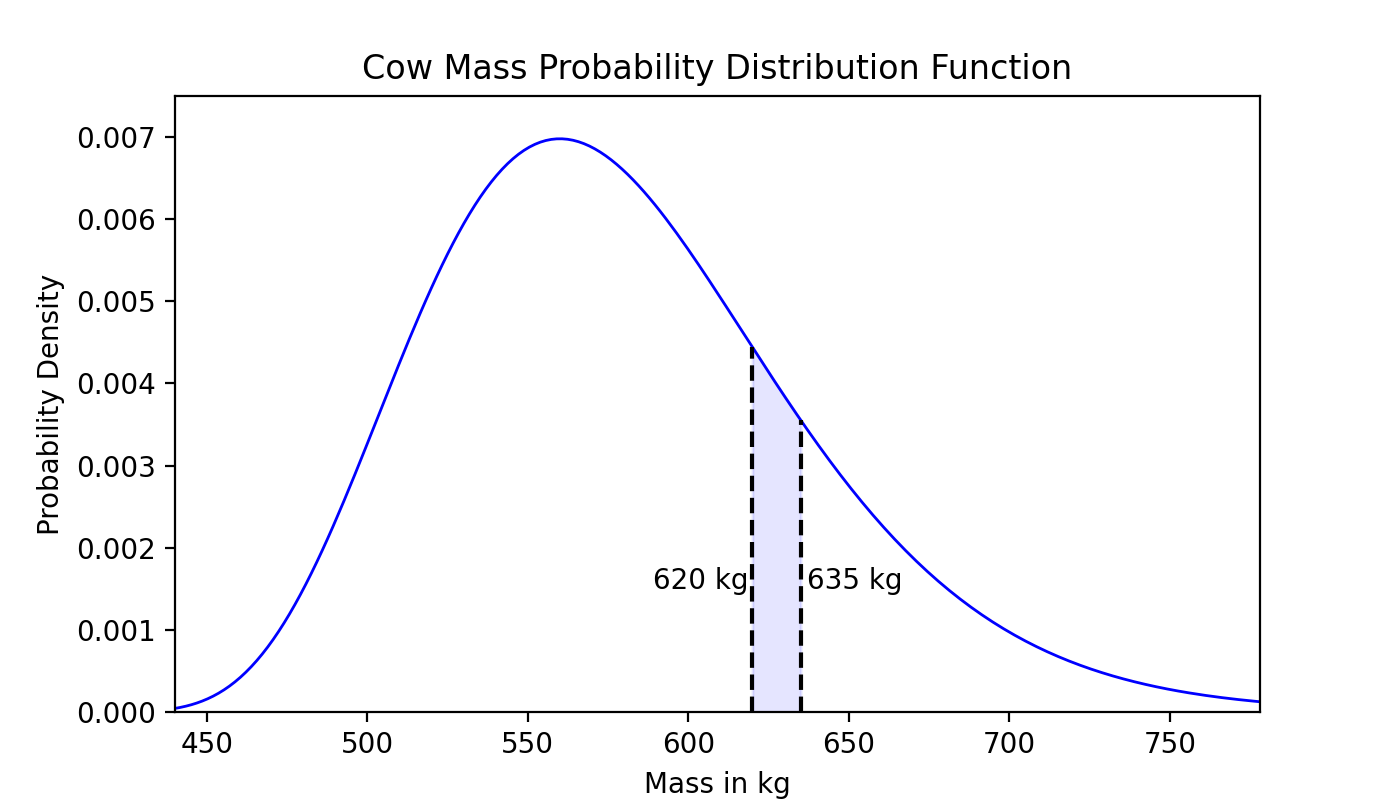
\includegraphics[width=0.7\textwidth]{cow_pdf_bounds.png}
    \caption{Probability density function with the integral from 620 kg to 635 kg.}
    \label{fig:cowpdfintegral}
\end{figure}

This is why it is called a "probability density" --- to get a true probability you need to multiply the density by the width of the region.

What is the area under the entire curve?  If you integrated it, you would get the CDF. The CDF goes from 0 to 1.0.  The area under a PDF is \emph{always} 1.0.

\subsection{The Continuous Uniform Distribution}\index{uniform distribution}

The most simple continuous distribution is the uniform distribution between two numbers $a$ and $b$. The CDF is a straight line from zero at $a$ to 1 at $b$. For example,
here is the CDF for the uniform distribution between 6 and 9:
\begin{figure}[H]
    \centering
    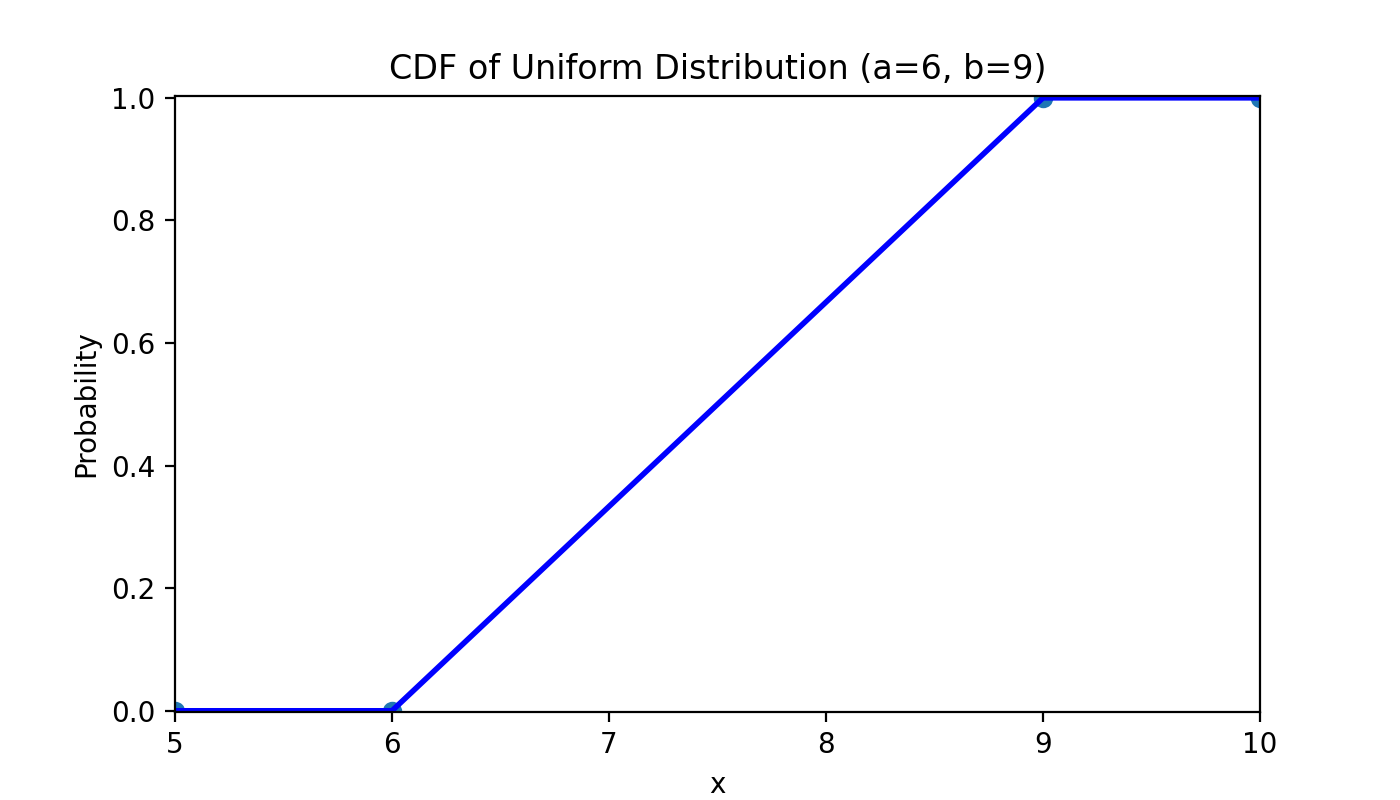
\includegraphics[width=0.7\textwidth]{unif_cdf.png}
    \caption{Cumulative distribution function for a uniform distribution between 6 and 9.}
    \label{fig:example_2-continuous_distributions}
\end{figure}

That line goes from 0 to 1 over a distance of 3, so its slope is $\frac{1}{3}$ between 6 and  9 and zero everywhere else. Thus, the PDF (its derivative) looks like this:
\begin{figure}[H]
    \centering
    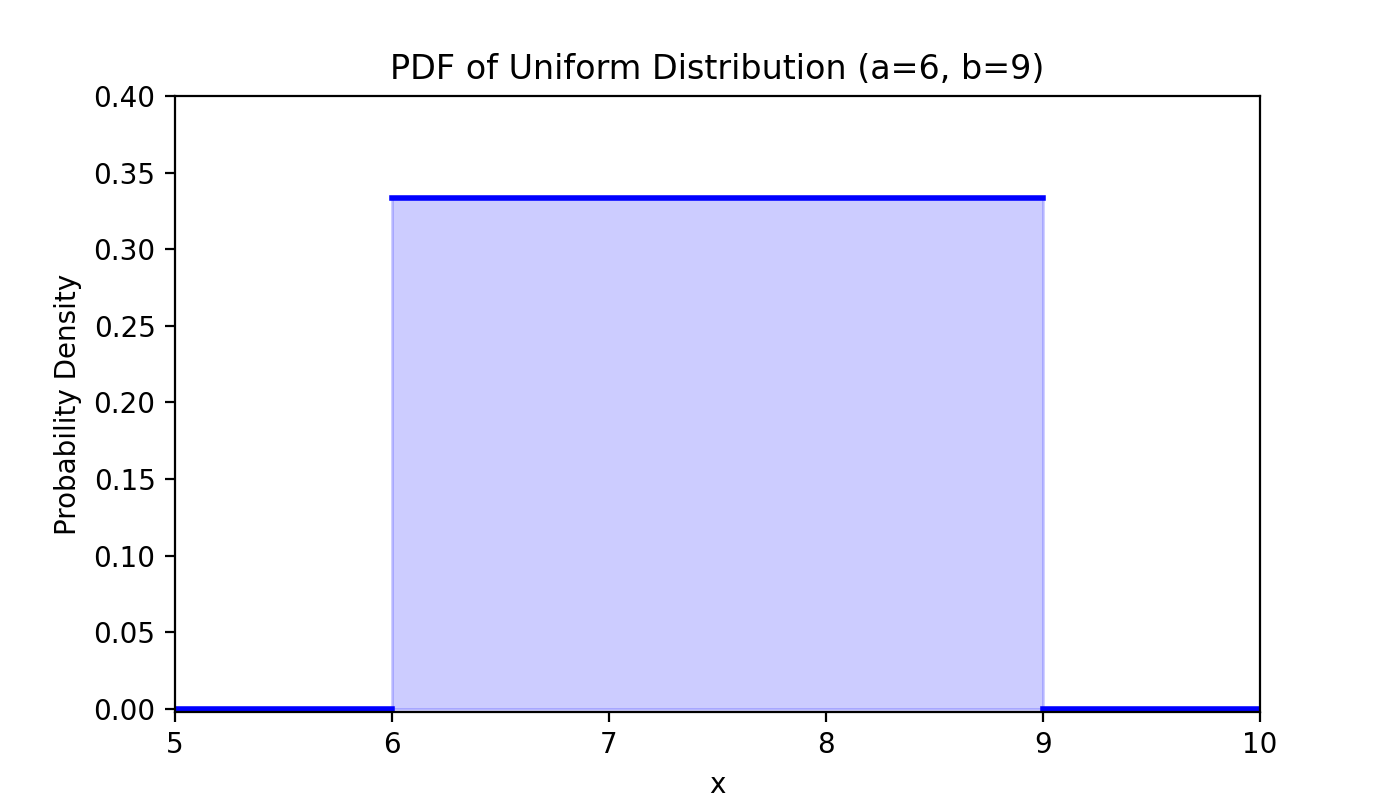
\includegraphics[width=0.7\textwidth]{unif_pdf.png}
    \caption{Probability density function for a uniform distribution from the continuous uniform distribution.}
    \label{fig:example_3}
\end{figure}

So, we can write the probability distribution of a continuous uniform distribution between $a$ and $b$ as:

  $p(x) = \begin{cases}
  \frac{1}{b-a} & \text{for } a \le x \le b, \\[8pt]
  0 & \text{for } x < a \ \text{ or } \ x > b.
  \end{cases}$

\index{probability density!versus probability}Notice that if $a$ and $b$ are less than 1 apart,  the value of $p(x)$ will be greater than 1. This is an important difference between a probability and a probability density: 
\begin{itemize}
\item A probability will always be in the interval $[0, 1]$. 
\item A probability density will never be less than 0,  but can be much larger than 1.
\end{itemize}

That said, the probability density will always integrate to 1.

Here is the PDF for a uniform distribution between 0.6 and 0.9:
\begin{figure}[H]
    \centering
    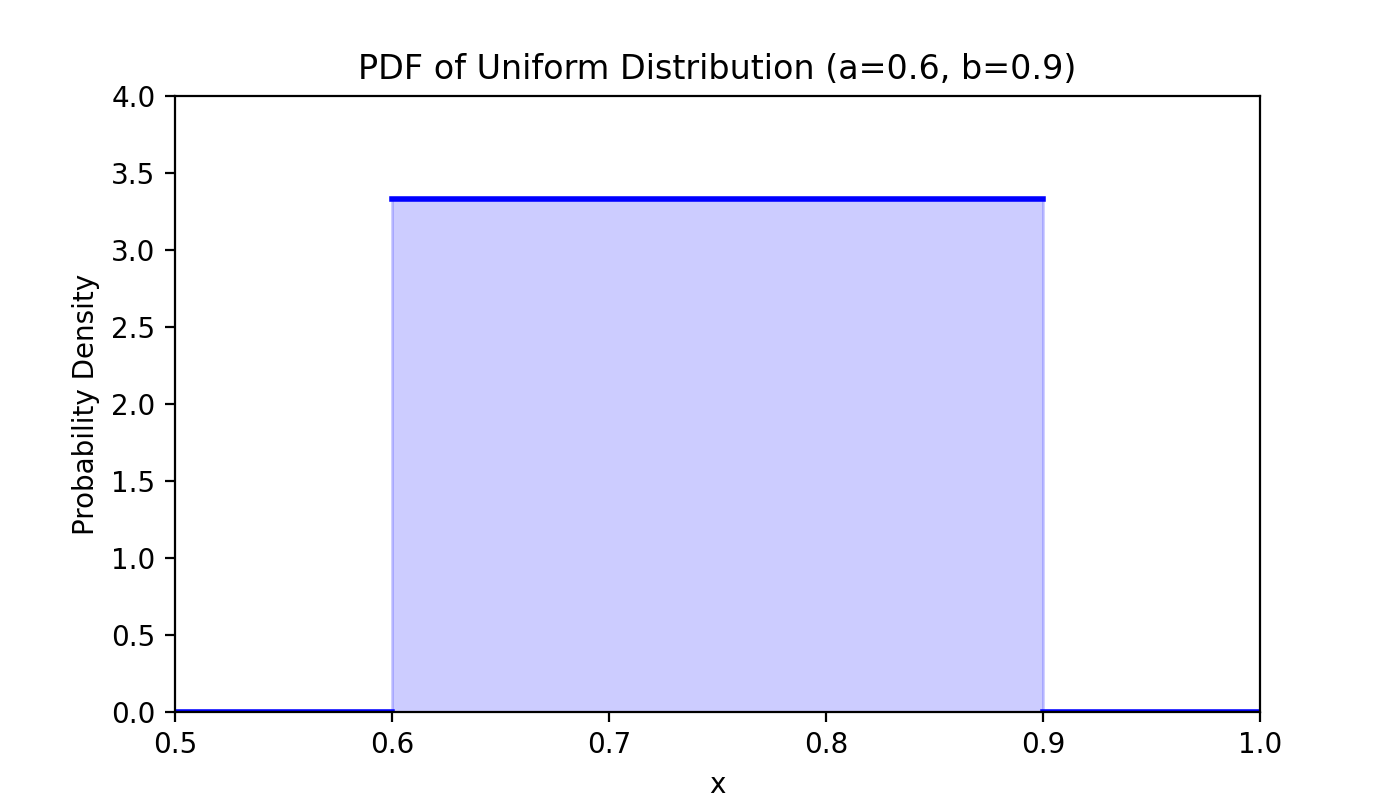
\includegraphics[width=0.7\textwidth]{unif_pdf2.png}
    \caption{Uniform probability density function.}
    \label{fig:unif_pdf2}
\end{figure}

The mean and median of a uniform distribution between $a$ and $b$ is its midpoint:  $\frac{a+b}{2}$.

The variance ($\sigma^2$) is $\frac{(b -a)^2}{12}$.

\subsection{Continuous Distributions In Python}
\index{cumulative distribution function!python}
The SciPy library has functions that let a programmer work with a large collection of different probability distributions.

For example,  if you wanted to work with a continuous uniform distribution between 6 and 9,  you would import the relevant
functions like this:

\begin{minted}{python}
from scipy.stats import uniform
\end{minted}

Now, if you wanted a numpy array containing a sample of 300 numbers generated randomly from that distribution:

\begin{minted}{python}
samples = uniform.rvs(loc=6,  scale=3,  size=300)
\end{minted}

The \pyvar{loc} argument is $a$. The \pyvar{scale} argument is $b - a$.

If you wanted to know the value of the probability density function at 8 and 10, you could use the \pyfunction{pdf} function:

\begin{minted}{python}
x_values = np.array([8, 10])
p_values  = uniform.pdf(x_values,  loc=6,  scale=3)
\end{minted}

Now, \pyvar{p\_values} contains 0.33333 and 0.0.

To get the value of the cumulative distribution function at those points,  you would use the \pyfunction{cdf} function:

\begin{minted}{python}
cdf_values = uniform.cdf(x_values,  loc=6,  scale=3)
\end{minted}

Now, \pyvar{cdf\_values} contains 0.666667 and 1.0.

The \index{inverse CDF}inverse of the CDF is very useful.  It answers questions like ``\index{percentile}How heavy does a cow have to be to be in top 1\%?''

\begin{minted}{python}
bottom_top_percentiles = np.array([0.01,  0.99])
boundaries = uniform.ppf(bottom_top_percentiles,  loc=6,  scale=3)
\end{minted}

Now, \pyvar{boundaries} contains 6.03 and 8.97.

The SciPy library supplies these functions (\pyfunction{rvs}, \pyfunction{pdf},  \pyfunction{cdf}, and \pyfunction{ppf}) for over a hundred 
common continuous probability distributions.  

The common "bell curve" shaped distribution is called a \index{Gaussian distribution}Gaussian  or Normal distribution. It is described by its mean (the midpoint of the bell) and its standard deviation.  For the normal distribution, about 68\% of the population lies within one standard deviation of the mean. 
We will talk a lot more about the normal distribution in other chapters,  but let us take this opportunity to plot the CDF and PDF of a normal distribution with a mean of 32 and a standard deviation of 8.

Create a file called \filename{plot\_norm.py} and add the following lines:

\begin{minted}{python}
import numpy as np
from scipy.stats import norm
import matplotlib.pyplot as plt

# Constants
MEAN = 32
STD = 8

# Plotting from the 0.5 percentile to the 99.5 percentile
x_min = norm.ppf(0.005, loc=MEAN, scale=STD)
x_max = norm.ppf(0.995, loc=MEAN, scale=STD)

# Make 200 points between x_min and x_max
x_values = np.linspace(x_min, x_max, 200)

# Get CDF for each x value
cdf_values = norm.cdf(x_values, loc=MEAN, scale=STD)

# Get PDF for each x value
pdf_values = norm.pdf(x_values, loc=MEAN, scale=STD)

# What is the highest density?
max_density = norm.pdf(MEAN, loc=MEAN, scale=STD)

# Make a figure with two axes
fig, axs = plt.subplots(nrows=2, sharex=True, figsize=(8, 8), dpi=200)
axs[0].set_xlim(left=x_min, right=x_max)

# Draw the CDF on the first axis
axs[0].set_title("CDF of Normal Distribution (mean=32, std=8)")
axs[0].set_ylim(bottom=0.0, top=1.0)
axs[0].plot(x_values, cdf_values)

# Draw the PDF on the second axis
axs[1].set_title("PDF")
axs[1].set_ylim(bottom=0.0, top=max_density * 1.1)
axs[1].plot(x_values, pdf_values)

# Add lines for mean,  mean-std, and mean+std
axs[1].vlines(MEAN - STD, 0, max_density, "r", linestyle="dashed")
axs[1].vlines(MEAN + STD, 0, max_density, "r", linestyle="dashed")

# Save out the figure
fig.savefig("norm_32_8.png")
\end{minted}

The resulting plot should look like this:

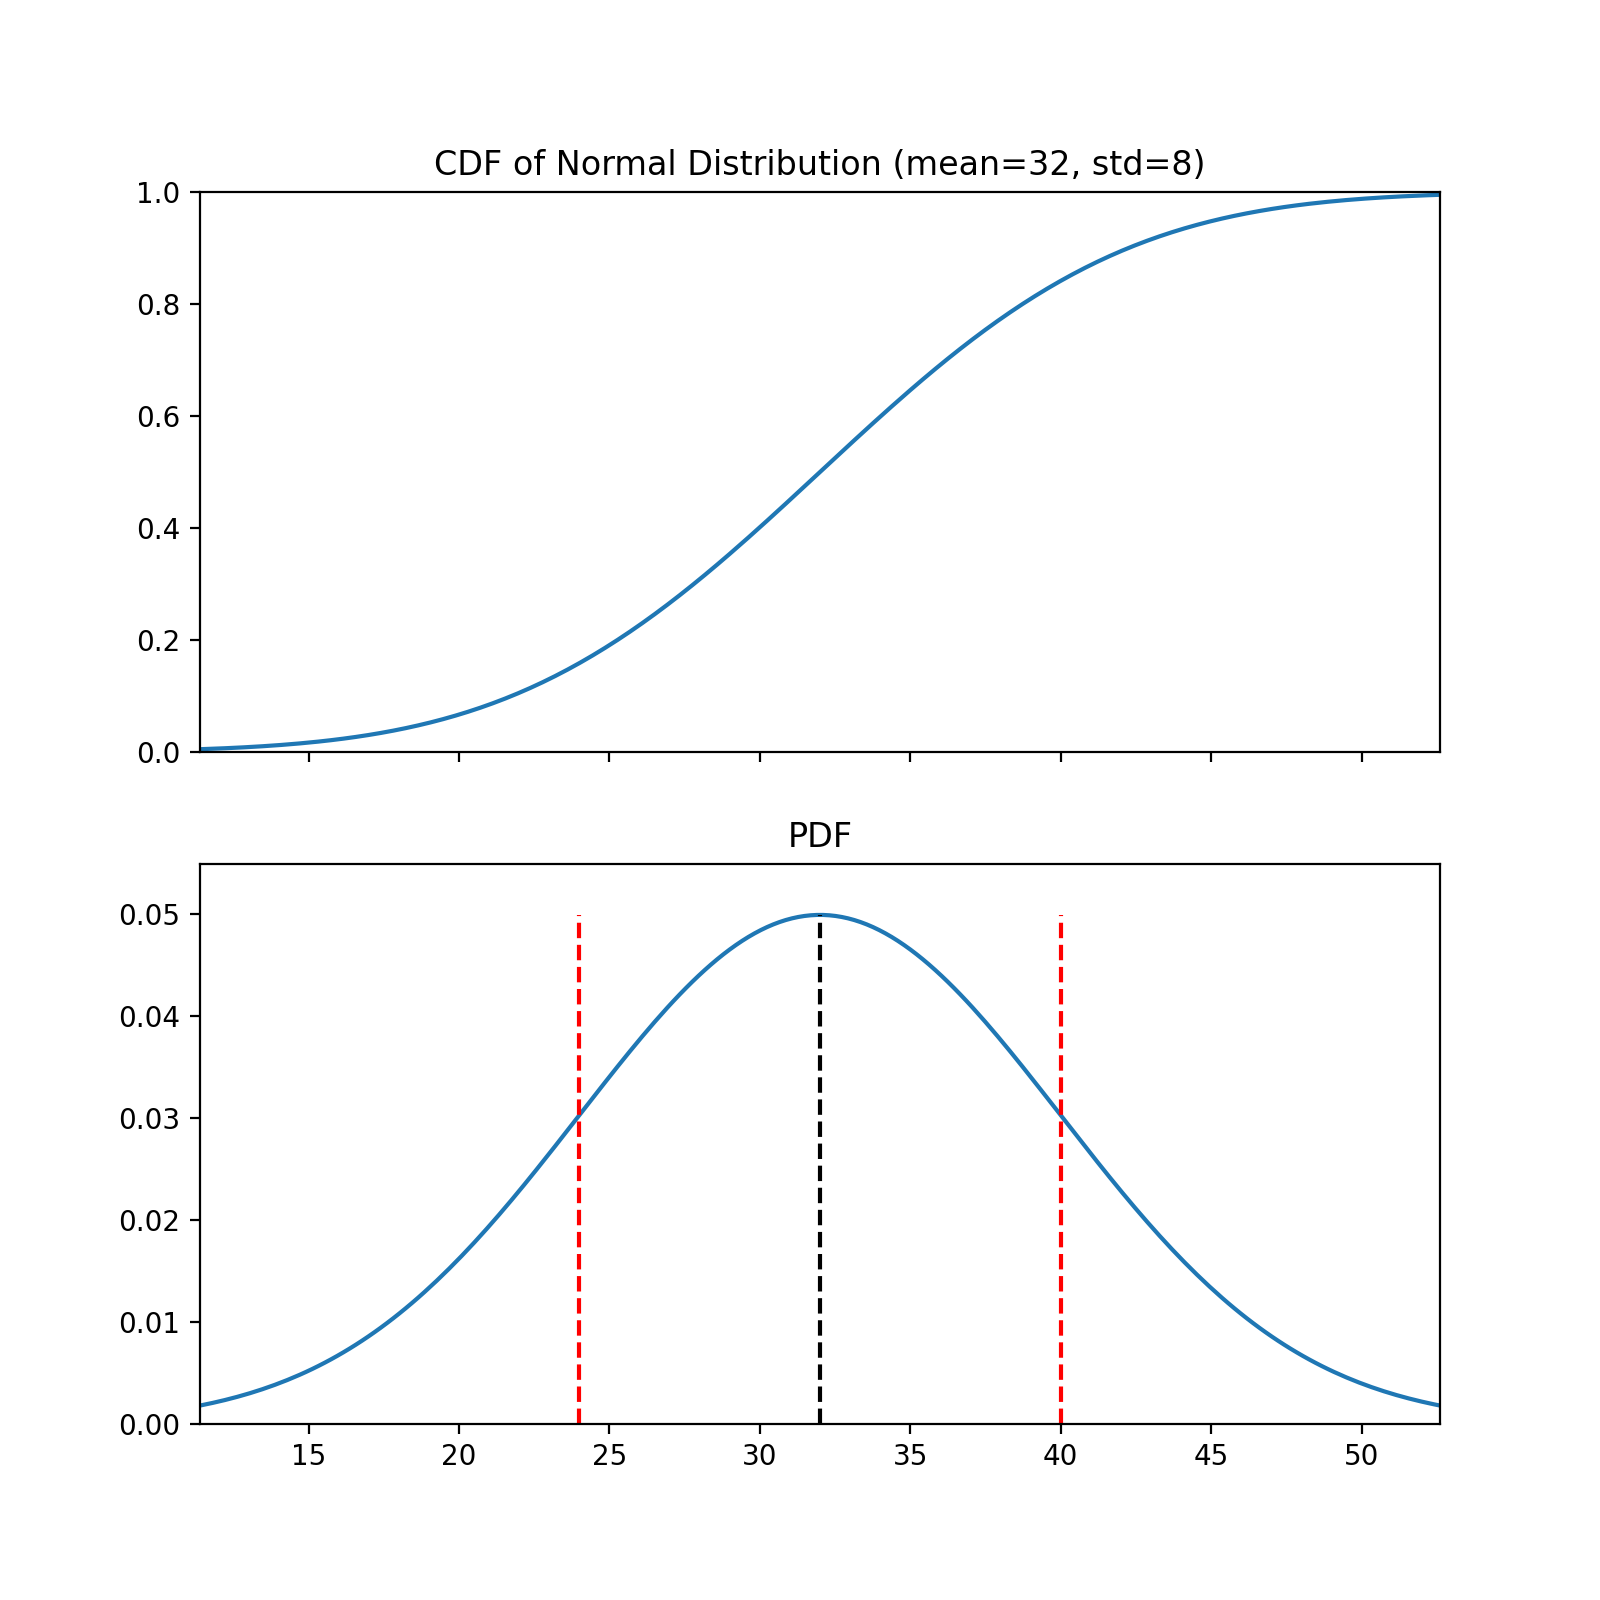
\includegraphics[width=0.7\textwidth]{norm_32_8.png}

What do those vertical lines mean?  An ornithologist might tell you, ``The wingspan of adult robins are normally distributed with a mean of 32 cm and a
 standard deviation of 8 cm.''  This means 68\% of the population of adult robins would have wingspans between the two red lines.
 
\begin{Exercise}[title={SciPy Stats}, label=scipy_ppf]

Globally,  the height of adult women is approximately normally distributed. The mean is 164.7 cm. The standard deviation is 7.1 cm.

Use Python and SciPy stats to answer these questions: 

\begin{itemize}
\item To be in the tallest decile (the top 10\%) of adult women,  how tall does one need to be? 

\item What percentage of adult women are between 160 cm and 165 cm?

\end{itemize}

(In case you are wondering: For men the mean is 178.4 cm and the standard deviation is 7.6 cm.)

\end{Exercise}
\begin{Answer}[ref=scipy_ppf]

\begin{minted}{python}
from scipy.stats import norm

# Constants
MEAN = 164.7 
STD = 7.1

# What is the cutoff for the top decile?
cutoff = norm.ppf(0.9, loc=MEAN, scale=STD);
print(f"To be in the top 10 percent, you must be at least {cutoff:.2f} cm")

# What proportion of women are between 160cm and 165cm?
shorter_than_160 = norm.cdf(160, loc=MEAN, scale=STD)
shorter_than_165 = norm.cdf(165, loc=MEAN, scale=STD)
between = shorter_than_165 - shorter_than_160
print(f"{between * 100.0:.2f}% of adult women are between 160 and 165 cm.")
\end{minted}

When run,  this will give you:

\begin{minted}{python}
> python3 women.py
To be in the top 10 percent, you must be at least 173.80 cm
26.29% of adult women are between 160 and 165 cm.
\end{minted}

\end{Answer}

\section{Probabilities as Areas}
Earlier in this chapter, you saw that for 
a single variable, $X$, the likelihood that variable $X$ has a certain value, 
$x$, is given by the probability distribution function (PDF), $f(x)$. 
Additionally, the total area under a PDF is always 1. Mathematically, this is 
because the PDF is the derivative of the cumulative density function (CDF), 
which always starts at 0 and ends at 1. Logically, the area under the PDF from 
$x = a$ to $x = b$ represents the likelihood that $X$ will be between $a$ and 
$b$. 

\begin{mdframed}[style = important, frametitle = {Probability that $X$ lies 
between $a$ and $b$}]
For a single variable, $X$, with a continuous density function, $f(x)$, the 
probability that $X$ lies between $a$ and $b$ is given by:
$$P( a \leq X \leq b) = \int_a^b f(x)\,dx$$
\end{mdframed}

Suppose that we know the PDF for human body mass and we wanted to know the 
probability that a randomly-selected person has a body mass between 70 and 80 
kgs. That probability would be represented by the integral of the PDF from $x 
= 70$ to $x = 80$ (see figure \ref{fig:mass_PDF}). 

\begin{figure}[H]
    \centering
    \begin{tikzpicture}
        \begin{axis}[axis lines = center, xmin = 0, xmax = 120, ymin = 0, 
        xlabel = mass (kg), ylabel = probability, clip = false]
            \addplot[name path = A, blue, thick, domain = 70:80]{
            (1/(10*sqrt(2*3.14159)))*(2.718)^(-1*(x - 72)^2/(2*10)^2)};
            \addplot[name path = B, black, thin, domain = 70:80]{0};
            \addplot[blue, thick, domain = 1:120, samples = 100] {
            (1/(10*sqrt(2*3.14159)))*(2.718)^(-1*(x - 72)^2/(2*10)^2)};
            \addplot[blue!30, opacity = 0.4] fill between [of = A and B];
            \draw[black, thin, dashed] (70, 0) -- (70, 0.04);
            \draw[latex-] (70, 0.035) -- (65, 0.04) node[left] {70 kg};
            \draw[black, thin, dashed] (80, 0) -- (80, 0.035);
            \draw[latex-] (80, 0.03) -- (90, 0.04) node[right] {80 kg};
        \end{axis}
    \end{tikzpicture}
    \caption{The highlighted area is equal to the probability that a person 
    has a mass between 70 and 80 kgs}
    \label{fig:mass_PDF}
\end{figure}

If we expand that integral to include all possible masses, what would the 
integral evaluate to? Since that would represent the probability that a random 
person has mass (which all people do), the integral should be equal to 1. In 
fact, the integral of a PDF over all possible values of the variable must be 
equal to 1, since that represents the sum of all the probabilities that the 
variable will hold all possible values. 

\begin{mdframed}[style = important]
For any probability density function, $f(x)$, the integral over the domain of 
$x$ is always 1.
$$\int_{-\infty}^{\infty} f(x)\,dx = 1$$
\end{mdframed} 

\textbf{Example}: Let $f(x) = kx(10-x)$ for $0 \leq x \leq 10$ and $0$ for all 
other values of $x$. Find a value for $k$. Then find the probability that $x$ 
lies between 7 and 10. 

\textbf{Solution}: Since $f(x)$ is a PDF, we know that:
$$\int_{-\infty}^{\infty} f(x)\,dx = 1$$

Solving for $k$:
$$1 = \int_{0}^{10} kx(10-x)\,dx = k\int_0^{10} 10x - x^2\,dx$$
$$= k \left[5x^2 - \frac{1}{3}x^3 \right]_{x = 0}^{x = 10} = k\left[500 - 
\frac{1000}{3} \right] = k \left( \frac{500}{3} \right) = 1$$

Which implies that $k = \frac{3}{500} = 0.006$

Therefore, in order to be a PDF, $f(x) = 0.006x(10-x)$ and we can find the 
probability that $X$ lies between 7 and 10:
$$P(7 \leq X \leq 10) = \int_7^{10} 0.006x(10 - x)\,dx$$
$$= 0.006 \left[5x^2 - \frac{1}{3}x^3 \right]_{x = 7}^{x = 10} = 0.006 \left[ 
5 \left(100 - 49 \right) - \frac{1}{3} \left(1000 - 343 \right) \right]$$
$$= 0.006 \left[ 255 - \frac{657}{3} \right] = 0.006(36) = 0.216 = 21.6\%$$

Therefore, there is a 21.6\% chance that $X$ lies between 7 and 10. 

\begin{Exercise}[title = {Representing Probabilities as Integrals}, 
label = rep_int]
Let $f(t)$ be the probability density function for the time it takes you to 
complete your weekly chores at home. Express the following probabilities as 
integrals or state what the given integral represents in words. 
\begin{enumerate}
\item that you spend less than 15 minutes on your chores.
\item that you spend between half an hour and an hour on your chores.
\item that you spend more than 45 minutes on your chores. 
\item $\int_{20}^{\infty} f(t)\,dt$
\item $\int_{60}^{120} f(t)\,dt$
\end{enumerate}
\end{Exercise}

\begin{Answer}[ref = rep_int]
\begin{enumerate}
\item $\int_0^{15} f(t)\,dt$
\item $\int_{30}^{60} f(t)\,dt$
\item $\int_{45}^{\infty} f(t)\,dt$
\item the probability that you spend more than 20 minutes on your weekly 
chores.
\item the probability that you spend between 1 and 2 hours on your weekly 
chores.
\end{enumerate}
\end{Answer}

\begin{Exercise}[title = {Using PDFs to Find Probabilities}, label = int_pdf]
For each $f(x)$, find $k$ such that $f(x)$ is a PDF. Then, find the requested 
probability. 
\begin{enumerate}
\item $f(x) = 
\begin{cases}
\frac{ke^{2 - x}}{\left(1 + e^{2 - x} \right)^2},&-2 \leq x \leq 6\\
0,&\text{otherwise}
\end{cases}$, $P(X \geq 2)$
\item $f(x) = \frac{k}{2 + 4x^2}$, $P(1 \leq X \leq 4)$
\item $f(x) = k(6x - 3x^2)$ for $0 \leq x \leq 2$ and 0 otherwise, $P(X > 3/4)$
\end{enumerate}
\end{Exercise}

\begin{Answer}[ref = int_pdf]
\begin{enumerate}
    \item We know that
	$$1 = \int_{-\infty}^{\infty} f(x)\,dx = \int_{-2}^{6} \frac{ke^{2 - x}}{
	\left( 1 + e^{2 - x} \right)^2}\,dx$$

	Let $u = e^{2 - x}$, then $-du = e^{2 - x}dx$. Substituting:
	$$= \int_{x = -2}^{x = 6} \frac{-k}{\left(1 + u \right)^2}\,du = k \left[
	 \frac{1}{1 + u} \right]_{x = -2}^{x = 6} = k \left[ \frac{1}{1 + e^{2 - x}} 
	 \right]_{x = -2}^{x = 6}$$
	$$= k \left[ \frac{1}{1 + e^{-4}} - \frac{1}{1 + e^4} \right] = \frac{k \left(
	e^4 - 1 \right)}{1 + e^4} = 1$$

	Which implies that $k = \frac{1 + e^4}{e^4 - 1}$. Substituting for $k$, we 
	find the probability that $X \geq 2$ is:
	$$P(X \geq 2) = \frac{1 + e^4}{e^4 - 1} \int_2^6 \frac{e^{2 - x}}{\left( 1 + 
	e^{2 - x} \right)^2}\,dx = \frac{1 + e^4}{e^4 - 1} \left[ \frac{1}{1 + e^{2 - 
	x}} \right]_{x = 2}^{x = 6}$$
	$$= \frac{1 + e^4}{e^4 - 1} \left( \frac{1}{1 + e^{-4}} - \frac{1}{1 + 1} 
	\right) = \frac{1 + e^4}{e^4 - 1} \left(\frac{1}{1 + e^{-4}} - \frac{1}{2} 
	\right) \approx 0.5$$

	There is a 50\% chance the variable will be greater than 2. 

    \item We know that:
    $$1 = \int_{-\infty}^{\infty} \frac{k}{2 + 4x^2}\,dx = \frac{k}{2} \int_{-
    \infty}^{\infty} \frac{1}{1 + 2x^2}\,dx$$
    $$= \frac{k}{2} \left[ \frac{\arctan{(\sqrt{2}x)}}{\sqrt{2}} \right]_{x = -
    \infty}^{x = \infty} = \frac{k}{2} \left[ \frac{\arctan{(\infty)}}{
    \sqrt{2}} - \frac{\arctan{(-\infty)}}{\sqrt{2}} \right] $$
    $$= \frac{k}{2} \left( \frac{\pi}{2\sqrt{2}} - \frac{-\pi}{2\sqrt{2}} 
    \right) = \frac{k}{2} \left( \frac{\pi}{\sqrt{2}} \right) = \frac{\pi k}{2
    \sqrt{2}} = 1$$

    Which implies that $k = \frac{2\sqrt{2}}{\pi}$. Therefore $f(x) = \frac{
    \sqrt{2}}{\pi \left(1 + 2x^2 \right)}$. Additionally, 
    $$P(1 \leq X \leq 4) = \int_1^4 \frac{\sqrt{2}}{\pi \left(1 + 2x^2 \right)
    }\,dx = \frac{\sqrt{2}}{\pi} \int_1^4 \frac{1}{1 + 2x^2}\,dx$$
    $$= \frac{\sqrt{2}}{\pi} \left[ \frac{\arctan{(\sqrt{2}x)}}{\sqrt{2}} 
    \right]_{x = 1}^{x = 4} = \frac{1}{\pi} \left[ \arctan{(4\sqrt{2})} - 
    \arctan{(\sqrt{2})} \right] \approx \frac{0.441}{\pi} \approx 0.140 = 14\%$$

    \item We know that:
    $$1 = \int_{-\infty}^{\infty} k \left(6x - 3x^2 \right)\,dx = 3k \int_{0}^{
    2} 2x - x^2\,dx$$
    $$= 3k \left[x^2 - \frac{1}{3}x^3 \right]_{x = 0}^{x = 2} = 3k \left( 4 - 
    \frac{8}{3} \right) = 3k \left( \frac{4}{3} \right) = 4k = 1$$

    Which implies that $k = 1/4$. And therefore,
    $$P(X > \frac{3}{4} ) = \int_{3/4}^2 \frac{6x - 3x^2}{4}\,dx = \frac{3}{4} 
    \int_{3/4}^2 2x - x^2\,dx$$
    $$= \frac{3}{4} \left[ x^2 - \frac{1}{3}x^3 \right]_{x = 3/4}^{x = 2} = 
    \frac{3}{4} \left[ (2)^2 - \left( \frac{3}{4} \right)^2 - \frac{1}{3} 
    \left( 2^3 - \left( \frac{3}{4} \right)^3 \right) \right]$$
    $$= \frac{3}{4} \left( \frac{175}{192} \right) = \frac{175}{256} \approx 
    68.4\%$$
\end{enumerate}
\end{Answer}

\subsection{Exponential PDFs}
There are two common PDFs used to model real-world probability distributions: 
exponential and normal distributions. We address exponential PDFs in this 
section and will discuss normal PDFs in the next. 

The time it takes for a radioactive particle to decay, or a bank teller to 
serve a customer, or a piece of equipment to fail are all commonly modeled 
with exponentially decreasing PDFs. These take the form:
$$f(t) = 
\begin{cases}
0,&\text{if }t<0\\
ce^{-ct},&\text{if }t \geq 0
\end{cases}$$

\textbf{Example}: Carbon-14 has a half-life of 5700 years, and the probability 
that a single particle will undergo decay after a given amount of time, $t$, 
is given by:
$$f(t) = 
\begin{cases}
    0,\text{ if}t<0\\
    \frac{1}{5700}e^{-t/5700}&\text{if }t \geq 0
\end{cases}$$

Where $t$ is in years. Find the probability that a particle of carbon-14 
decays before 5700 years. 

\textbf{Solution}: 
$$P(T \leq 5700) = \int_0^{5700} \frac{1}{5700} e^{-t/5700}\,dt$$
$$= \frac{1}{5700} \left(-5700 \right) \left[e^{-t/5700} \right]_{t = 0}^{
t = 5700}$$
$$= -1 \left[ e^{-1} - e^{0} \right] = 1 - \frac{1}{e} \approx 63.2\%$$

The next chapter is about the most important continuous distribution of all: the normal distribution.
